\chapter{Conexión}%
\label{cha:conexion}
\section{Concepto y mantras}%
\label{sec:concepto_y_mantras_conx}
\begin{defi}[Conexión]
Sea $X$ un espacio topológico, decimos que es \textbf{conexo} si y sólo si cumple las siguientes condiciones equivalentes:
\begin{enumerate}
    \item $\nexists U,V \stackrel{ab.}{\subsetneq} X: X= U \sqcup V$ donde $U$ y $V$ son no vacíos y disjuntos.
    \item $\nexists F,C \stackrel{cerr.}{\subsetneq} X: X= F \sqcup C$ donde $F$ y $C$ son no vacíos y disjuntos.
    \item $\nexists E \subsetneq X$ no vacío que sea abierto y cerrado simultáneamente.
\end{enumerate}
\end{defi}
\begin{demo}
Equivalencia: $F = \underbrace{X \setminus V}_{= U},\ C = \underbrace{X \setminus U}_{= V},\ E = U = X \setminus V.$
\end{demo}

\begin{obs}
Si quisiéramos estudiar la conexión de un subespacio no como un espacio en sí mismo sino en términos relativos al espacio ambiente inicial, bastaría con dar la siguiente definición:
\[
\nexists U,V \ab X : Y \subset U \cup V \mbox{ y } \begin{cases}
    U \cap Y \neq \emptyset\\
    V \cap Y \neq \emptyset\\
    U \cap V \cap Y = \emptyset
\end{cases} 
\]
y esta sería equivalente a estudiar la conexión en $Y$ con su topología relativa, esto es, como espacio topológico en sí mismo.
\end{obs}

\begin{ej}
\begin{itemize}
    \item El espacio real usual $\mathbb{R}$ es conexo.
    \item El espacio de los racionales $\mathbb{Q}$ con la topología usual no es conexo y , de hecho, es \textbf{totalmente disconexo} porque los únicos conexos son los puntos.
    \begin{demo}
        %TODO: Dibujo y el hace algo con Y \subset Q
        %Hay que ver que el único subespacio conexo es {q} q in Q
        Si dividimos $\mathbb{R}$ en dos segmentos disjuntos separados por $\alpha \in \mathbb{R} \setminus \mathbb{Q}$ tenemos que $\mathbb{Q} = \mathbb{Q} \cap \left( \left[ -\infty, \alpha \right) \sqcup \left( \alpha, +\infty \right] \right)$ que son abiertos en $\mathbb{Q}$ y disjuntos.
    \end{demo}
    \item En $\mathbb{R}$ con la topología \textit{Sorgenfrey} sólo son conexos los puntos, es decir, es totalmente disconexo.
    \item El intervalo $\left( 0, 1 \right)$ con la topología usual es conexo. 
    \item En general, los segmentos en $\mathbb{R}^n$, los estrellados y los convexos son conexos.
\end{itemize}
\end{ej}

\begin{theo}[del pivote] 
Sea $X$ un espacio topológico y $A$ un conjunto definido como $A := \bigcup_{i\in I} A_i$ donde los $A_i$ son una familia de conexos en $X$, si se da alguna de las siguientes condiciones:
\begin{enumerate}
\item $\bigcap_{i \in I} A_i \neq \emptyset$.
\item $\exists i_0 \in I : \forall i \in I, \ A_{i_0}\cap A_i \neq \emptyset$.
\item $\forall i \in I: A_i \cap A_{i+1} \neq \emptyset$.
\end{enumerate}
entonces el conjunto $A$ es conexo.
\end{theo}
\begin{demo}
\begin{enumerate}
\item Para demostrar la primera implicación, podemos ver que cualquier conjunto $E\subset A$ no vacío que sea abierto y cerrado simultáneamente ha de ser $A$.

En primer lugar, hay que tener en cuenta que $E\cap A_i \ac A_i$ y, como estos son conexos, sólo hay dos alternativas: $E\cap A_i = \emptyset$ o $E\cap A_i = A_i$. No puede ocurrir que $\forall i \in I:  E \cap A_i = \emptyset$ porque entonces $E\cap \bigcup_{i\in I}A_i = \emptyset$, es decir, $E\cap A= \emptyset$ lo que sería absurdo. Así pues, podemos decir que $\exists i_0\in I : A_{i_0}\cap E = A_{i_0}$ y, como $P:= \bigcap_{i\in I} A_i \neq \emptyset$ y $P\subset E$ sabemos que todos los demás $A_i\cap E$ deben ser necesariamente $A_i$ pues no pueden ser vacíos ya que $\emptyset \neq P \subset A_i \cap E$.

De esta manera, hemos conseguido ver que $E \supset E\cap A_i = A_i$ y entonces $A = \bigcup_{i\in I}A_i \subset E \Rightarrow A=E$, es decir, $A$ es conexo.

\item Para demostrar la segunda implicación, basta con aplicar la primera que ya ha sido demostrada.

Como la intersección $A_{i_0}\cap A_i$ es no vacía y ambos conjuntos son conexos, por la primera implicación la unión $B_i := A_{i_0}\cup A_i$ es conexa. De esta manera, podemos escribir el total como
\[
A= \bigcup_{i\in I}A_i = \bigcup_{i\in I}\underbrace{A_i\cup A_{i_0}}_{B_i} \mbox{ donde }\bigcap_{i\in I} B_i = A_{i_0} \neq \emptyset
\]
así que podemos decir que es conexo por la primera implicación.

\item Para $A_1$ y $A_2$, como la intersección es no vacía y ambos son conexos, por la primera implicación la unión $A_1 \cup A_2 =: B_2$ es conexa. Si ahora miramos $B_2$ y $A_3$, vemos que la intersección es no vacía (pues $A_2 \cap A_3\neq \emptyset$) y, como ambos son conexos, la unión $B_3 := B_2 \cup A_3$ es conexa. De esta manera y de forma inductiva, se llega a que la unión de todos es conexa, es decir, que $A$ es conexo.
\begin{figure}[H]
            \centering
            \incfig[0.5]{cadena-de-conexos}
            \caption{\textit{Ejemplo de una cadena de conexos.}}
            \label{fig:cadena-de-conexos}
\end{figure}
\end{enumerate}
\end{demo}

\begin{prop}[Construcción de cadenas]
Sea $X$ conexo tal que $X = \bigcup_{i \in I} U_i$, recubrimiento abierto y $p, q \in X \Rightarrow \exists U_{i_0} \cup \ldots \cup U_{i_k}$ de $p$ a $q: p \in U_{i_0}, U_{i_{k - 1}} \cap U_{i_k} \neq \emptyset,\ q \in U_{i_r}$. 
\end{prop}
\begin{demo}
Veamos que $A = \{x \in X: \exists U_{i_k} \text{, cadena, de } p \text{ a } x\} \neq \emptyset$ abierto y cerrado $\Rightarrow A = X$ y $q \in A$, es decir, para cualquier elemento de $X$ existe una cadena desde $p$ que es lo que buscamos. Esto se debe a que: 
\begin{itemize}
    \item \underline{No vacío}: $\exists U_{i_0} \ni p$ y $U_{i_0}$ va de $p$ a $p$.
    \item \underline{Abierto}: $\exists U_{i_0}, \ldots, U_{i_r}$ de $p$ a $x \Rightarrow U_{i_r} \subset A$, es decir, es entorno de todos sus puntos.
    \item \underline{Cerrado}: 
    \begin{align*}
        y \in \overline{A} \text{ e } y \in U_{i\left( y \right)} &\Rightarrow A \cap U_{i\left( y \right)} \neq \emptyset\\
        &\Rightarrow \exists U_{i_0}, \ldots, U_{i_r} \text{ de } p \text{ a } x\in U_{i\left( y \right)}\\
        &\Rightarrow U_{i_0}, \ldots, U_{i_r}, U_{i\left( y \right)} \text{ de } p \text{ a } y
    .\end{align*}
    Por tanto, $y \in A$, es decir, $A = \overline{A}$.
\end{itemize}
%TODO: Imagen
\begin{center}
    \includegraphics[scale=0.3]{images/dem_const_cadenas} 
\end{center}
Con esto es un subconjunto de uno conexo, no vacío, abierto y cerrado, es decir, es el total.
\end{demo}

\begin{prop}[Mantra 2]
Sean $X$ e $Y$ espacios topológicos, $X$ conexo y $f:X\rightarrow Y$ una aplicación continua entre ambos espacios, entonces $f(X)$ es conexo.
\end{prop}
\begin{demo}
Escogemos un conjunto $E \ac f\left( X \right)$ no vacío en la imagen. La preimagen $f^{-1}\left( X \right)$ es no vacía, abierta y cerrada en $X$ por la continuidad de la función $f$ y, como $A$ es conexo entonces $f^{-1}\left( E \right) = X$, lo que quiere decir que $E = f\left( X \right)$.
\end{demo}

\begin{prop}[Mantra 3]
Sea $X$ un espacio topológico y $A\subset X$ un subconjunto conexo, la adherencia $\overline{A}$ es un conjunto conexo.
\end{prop}
%TODO queda por hacer esta demostración que no entiendo, pues recurre a la densidad (que en las hipótesis no se menciona).
\begin{demo}
La demostración puede hacerse a través del hecho de que si $Y\subset X$ es denso en $X$ y $Y$ es conexo, entonces $X$ es conexo, pues si esto está demostrado $A\subset \overline{A}$ y todo conjunto es denso en su adherencia.

De esta manera y suponiendo $Y \subset X$ denso y $Y$ conexo, tomamos un conjunto
\[
\emptyset \neq E \ac X \Rightarrow \underbrace{E \cap Y}_{\neq \emptyset} \ac Y \Rightarrow E \cap Y = Y \Rightarrow Y \subset E \cerr X = \overline{Y} \Rightarrow E = X
\]
\end{demo}

\begin{obs}
El resultado anterior es importante por el hecho de que permite demostrar que un conjunto es conexo a través de la conexión de un subconjunto denso. Como la adherencia es el total, si el conjunto denso es conexo, el total también lo es.
\end{obs}

\begin{ej}
   %TODO: Ejemplos complicados
\begin{enumerate}
    %TODO: Ejemplo de la esfera y del proyectivo.

    \item Como el intervalo $\left( 0, 1 \right)$ es denso en el intervalo $\left[ 0, 1 \right]$ (pues se trata de su adherencia), entonces $\left[ 0, 1 \right]$ conexo.
    
    \item Sabiendo que $[0,1]$ es conexo, podemos generalizar el razonamiento anterior a través de otro método: viendo que la aplicación $\sigma\left( t \right) = \left( 1 - t \right) a + tb$ establece un homeomorfismo con $\left[ a, b \right] \subset \mathbb{R}^n$ y, por ser continua y $[0,1]$ conexo, entonces $\left[ a, b \right]$ es conexo.
    
    \item Con aún más generalidad y conociendo los casos anteriores, podemos deducir que otros conjuntos también son conexos:
    \begin{itemize}
        \item Los conjuntos estrellados $E = \bigcup_{\substack{x \in E\\ \text{conx.}}} \left[ a, x \right]$ respecto de $a$, los convexos, las bolas abiertas y cerradas, los rectángulos... son todos conexos gracias al teorema del pivote y los resultados anteriores.
        
        \item Las trazas de curvas continuas $\sigma: \left[ 0, 1 \right] \rightarrow \mathbb{R}^n$ tales como caminos, etc. son conexos, pues son imagen continua de conexos.
    \end{itemize}
    
    \item Seno del topólogo/polaco:
    
    Si uno considera la función $f(t) = sen(1/t)$ la gráfica que observa es la que se ve en la figura \ref{fig:seno_topologo}. Dicha gráfica, que denotaremos por $\Gamma$ es un conjunto conexo, pues es imagen continua de un conexo. La línea vertical donde se ``aprieta'' la función, que denotaremos por $J$, también lo es por ser un segmento (más bien homólogo a uno). Lo interesante es que la unión de ambas cosas es conexa pues precisamente es la adherencia de la gráfica $J$.

    \begin{figure}[H]
        \centering
        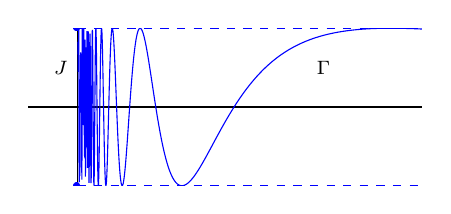
\begin{tikzpicture}
        \begin{axis}[
            axis lines* = middle,
            height=2cm,
            width=5cm,
            scale only axis=true,
            ytick=\empty,
            xtick=\empty,
            xmin=-0.1,
            xmax=0.7,
            ymin=-1,
            ymax=1,
        ]
        \addplot[
            domain=0.001:0.8,
            samples=1000,
            color=blue,
            smooth,
        ]
        {sin(deg(1/x))};
        \draw[blue, dashed] (0,1) -- (1,1);
        \draw[blue, dashed] (0,-1) -- (1,-1);
        \node at (0,0.5) [left] {\scriptsize $J$};
        \node[blue] at (0,1) {\tiny \textbullet};
        \node[blue] at (0,-1) {\tiny \textbullet};

        \node at (0.5, 0.5) {\scriptsize $\Gamma$};
        \end{axis}
        \end{tikzpicture}
        \caption{\textit{Seno del topólogo o de Varsovia.}}
        \label{fig:seno_topologo}
    \end{figure}
\end{enumerate}
\end{ej}

\section{Tabla de comportamiento}%
\label{sec:tabla_de_comportamiento_conx}
En este apartado estudiamos como comporta la propiedad definida con respecto a las construcciones del tema \nameref{cha:construcciones}. Se trata de ver cuándo se conserva, cuándo no y qué hipótesis podemos añadir para que se conserve en los casos que no.

\begin{table}[H]
\centering
\begin{tabular}{| c | c | c | c | c |}
\hline
& Subespacios & Cocientes & Productos & Sumas\\
\hline
    Conexión & \ding{55} & \checkmark & \checkmark & \ding{55} \\
    \hline
    Demostración: & $\{0, 1\} \subset \left[ 0, 1 \right]$ & Mantra $3$ & Pivote & Cada sum. es ab. y cerr.\\
    \hline
\end{tabular}
\caption{\textit{Tabla de comportamiento de la conexión con respecto a las construcciones.}}
\end{table}

\begin{prop}
$X \times Y$ conexo $\Leftrightarrow X$ y $Y$ conexo.
\end{prop} 
\begin{demo}
\begin{itemize}
    \item[$\Rightarrow)$] Cada factor es imagen del total a través de la función proyección, que es continua. Como el total es conexo, la imagen continua a través de un conexo es conexa, luego se tiene el resultado.

    \item[$\Leftarrow)$] Fijamos un valor $a \in X$ y entonces vemos que el conjunto
    \[
    Z_y = \underbrace{\left( X \times \{y\} \right)}_{\approx X}\cup \underbrace{\left( \{a\} \times Y \right)}_{\approx Y}
    \]
    es conexo por ser dos conexos que se cortan en el punto $\left( a, y \right)$ (teorema del pivote).
    
    Además, la intersección de todos los $Z_y$
    \[
    \bigcap_{y \in Y} Z_y = \{a\} \times Y \neq \emptyset
    \]
    es no nula, luego por el teorema del pivote de nuevo, tenemos que:
    \[
    \bigcup_{y \in Y} Z_y = X \times Y \text{ conx.}
    \]
    \begin{figure}[H]
        \centering
        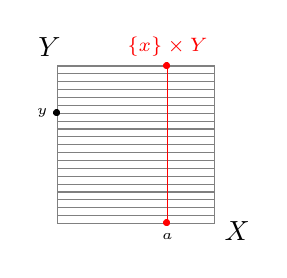
\begin{tikzpicture}
            \draw[gray] (0,0) rectangle (2,2);
            \foreach \y in {0.1, 0.2, ..., 2}
                {
                    \draw[gray,-] (0,\y) -- (2,\y);
                }
            \node at (0,1.4) {\tiny\textbullet};
            \node at (0,1.4) [left] {\tiny $y$};

            \node[red] at (1.4,0) {\tiny\textbullet};
            \node at (1.4,0) [below] {\tiny $a$};

            \draw[red,-] (1.4,0) -- (1.4,2);
            \node[red] at (1.4,2) {\tiny\textbullet};
            \node[red] at (1.4,2) [above] {\scriptsize $\left\{ x \right\} \times Y$};

            \node at (-0.1,2) [above] {$Y$};
            \node at (2,-0.1) [right] {$X$};
        \end{tikzpicture}
        \caption{\textit{Representación de que el producto conexos es conexo: cada línea del cuadrado es un $X \times \left\{ y \right\}.$}}
    \end{figure}
\end{itemize}
\end{demo}


\chapter{Componentes conexas y\texorpdfstring{\\}{} conexión local}%
\label{cha:componentes_conexas_y_conexion_local}
\section{Componentes}%
\label{sec:componentes}
\begin{defi}
Una \textbf{componente conexa} (c.c) de $X$ es un subespacio conexo maximal.
\end{defi}

\begin{prop}[Construcción]
\begin{enumerate}
    \item $\forall a \in X$ definimos: $C\left( a \right) = \bigcup_{a \in A \text{conx.}} A$ es conexo (por t. pivote), $a \in C\left( a \right)$.
    \item $E \subset X$ conexo tal que $C\left( a \right) \cap E \neq \emptyset \Rightarrow$
    \[
    C\left( a \right) \cup E \text{ conx. (pivote)} \Rightarrow C\left( a \right) \cup E \text{ es uno de los } A \text{ de } C\left( a \right) \Rightarrow E \subset C\left( a \right) 
    \]
    Luego, 
    \begin{itemize}
        \item $C\left( a \right)$ maximal $\Rightarrow$ componente conexa.
        \item $a \neq b: C\left( a \right) = C\left( b \right)$ ó $C\left( a \right) \cap C\left( b \right) = \emptyset$. Usamos $E = C\left( b \right)$.
    \end{itemize}

    \item $\overline{C\left( a \right)}$ conexo (mantra adh.) $\Rightarrow \overline{C\left( a \right)} = \underbrace{C\left( a \right)}_{\text{cerr.}}$ (maximalidad)
    %TODO: Fix
    \item[1. + 2. + 3.] $\Rightarrow X = \bigsqcup_{C \stackrel{\text{c.c}}{\subset}  X} C$ es una \underline{partición} de cerrados disjuntos.
\end{enumerate} 
\end{prop}

\begin{ej}
\begin{enumerate}
    \item $X_{\text{discreto}}: C\left( x \right) = \{x\}$ (puntos abiertos y cerrados)
    \item $\mathbb{Q}_u : C\left( p \right) = \{p\}$ (todo intervalo de $\mathbb{R}$ tiene racionales)
    \item $\left( \mathbb{R}, \mathcal{T}_{[, )} \right): C\left( t \right) = \{t\}$ ($\mathbb{R} = \left( \leftarrow, a \right) \cup \left[ a, \rightarrow \right)$ abierto y cerrado)
    \item $X = \{0, Y_k,\ k \ge 1\} : \begin{cases}
        C\left( 0 \right) = \{0\} \text{ cerrado, no abierto} \left( \{\frac{1}{k}: k\ge 1 \}  \text{ no cerr.}\right)\\
        C\left( \frac{1}{k} \right) = \{\frac{1}{k}\} \text{ cerrado y abierto.} 
    \end{cases} $
\end{enumerate}
\end{ej}

\begin{defi}
Un espacio cuyas componentes son los puntos se llama \textbf{totalmente disconexo}. 
\end{defi}

\begin{prop}
Las componentes conexas de $X \times Y$ son los productos de componentes conexas.
\end{prop}
\begin{demo}
$C \stackrel{\text{c.c}}{\subset} \underbrace{X}_{\xrightarrow{p} X} \times \underbrace{Y}_{\xrightarrow{q} Y} \Rightarrow p\left( C \right)$ y $q\left( C \right)$ conexos en $X$ e $Y$, respectivamente, (imagen continua) $\Rightarrow \begin{cases}
    p\left( C \right) \subset E \stackrel{\text{c.c}}{\subset}  X\\
    q\left( C \right) \subset F \stackrel{\text{c.c}}{\subset}  Y
\end{cases} \Rightarrow C \subset E \times F \xRightarrow{\text{Max. de } C} C = E\times F$.
\end{demo}

\section{Conexión local}%
\label{sec:conexion_local}
\begin{defi}
$X$ es \textbf{localmente conexo}  si $\forall x \in X,\ \exists \mathcal{B}^x$ base de entornos abiertos conexos.
\end{defi}

\begin{prop}
$X$ es localmente conexo $\Leftrightarrow$ las componentes conexas de un abierto son abiertas:
\[
U \ab X \text{ y } C \stackrel{\text{c.c}}{\subset} U \Rightarrow C \ab X.
\]
\end{prop}
\begin{demo}
\begin{itemize}
    \item[$\Rightarrow)$] Si $x \in C \stackrel{\text{c.c}}{\subset} U \ab X \Rightarrow \exists \underbrace{U^x}_{\text{ab. conx.}} \subset U \Rightarrow U^x \subset C \Rightarrow C \ab X$. Es decir, $U$ es entorno de todos sus puntos.
    \item[$\Leftarrow)$] $ \mathcal{B}^x = \{C\left( x \right) \stackrel{\text{c.c}}{\subset} U \ab X : x \in U\}$. Con $C\left( x \right)$ abierto por ser c.c de abierto.
\end{itemize}
\end{demo}

\begin{enun}
$X$ es localmente conexo $\Leftrightarrow \forall x \in X,\ \exists \mathcal{V}^x$ base de entornos conexos.
\end{enun}

\begin{ej}[Esencial]
$\{0, \frac{1}{k} : k \ge 1\} = Y \subset \mathbb{R}_u$ \underline{no} es localmente conexo. 
\begin{demo}
    La $\text{c.c}\left( 0 \right) = \{0\}$ no es abierto. Directamente:
    \begin{align*}
        0 \in \underbrace{V}_{\text{ent. de } 0 \in \mathbb{R}} \cap Y &\Rightarrow V \supset \left( 0, \varepsilon \right),\ \exists 0 < \underbrace{\theta}_{\not\in \mathbb{Q}} < \frac{1}{k} < \varepsilon < 1\\
        &\Rightarrow V\cap Y \subset \underbrace{\left( \leftarrow, \theta \right)}_{\ni 0} \cup \underbrace{\left( \theta, \rightarrow \right)}_{\ni \frac{1}{k}}  \Rightarrow V \cap Y \text{ no conexo.} 
    .\end{align*}
\end{demo}
\end{ej}

\begin{enun}
\begin{enumerate}
    \item Analizar una sucesión de segmentos que convergen a otro:
    \begin{figure}[H]
        \centering
        \begin{tikzpicture}
            \foreach \x in {0, 0.005, 0.01, 0.02, 0.035, 0.1, 0.25, 0.5, 0.8, 1.5, 3, 6}
                \draw[-, gray] (\x, 0) -- (\x, 2);
        \end{tikzpicture}
        \caption{\textit{Ejemplo}}
    \end{figure}
    \item ¿Y el seno del topólogo?
\end{enumerate}
\end{enun}

\section{Tabla de comportamiento}%
\label{sec:tabla_de_comportamiento_loc_conx}
%TODO: Fix tabla. En subespacios los abiertos sí heredan
\begin{table}[H]
\begin{tabular}{| c | c | c | c | c |}
\hline
& Subespacios & Cocientes & Productos & Sumas\\
\hline
Conexión local & \ding{55} & \checkmark & \checkmark & \checkmark\\
\hline
Demostración: & Ejemplo esencial & No banal & Prod. ent. conx. & Suma como sum's\\
\hline
\end{tabular}
\caption{\textit{La tabla nos indica como se conserva la compacidad local en las construcciones que hemos visto. Las sumas y los productos son finitos.}}
\end{table}


\begin{prop}
Sea $f : X \rightarrow Y$ identificación con $X$ localmente conexo $\Rightarrow Y$ es localmente conexo.
\end{prop}
\begin{demo}
    El diagrama siguiente resume el argumento (si se lee en el orden adecuado).
    \begin{center}
        \includegraphics[scale=0.3]{images/dem_loc_conx_loc_conx} 
    \end{center}
\end{demo}
